\documentclass[30pt,extrafontsizes]{memoir}
%\setstocksize{30in}{40in}
\usepackage{xcolor}
\usepackage[paperwidth=40in,paperheight=30in,margin=1.25in]{geometry}
\pagestyle{empty}

%\usepackage[default,semibold]{sourcesanspro}
%\usepackage{sourcecodepro}
%\usepackage[T1]{fontenc}
\usepackage{fontspec}
%\setmainfont[BoldFont={Source Sans Pro Semibold}]{Source Sans Pro Light}
\setmainfont[BoldFont={Source Sans Pro Semibold}, RawFeature={+kern, +ss01}]{Source Sans Pro}

\usepackage[english]{babel}
\usepackage{blindtext}

\usepackage{pbox}
\usepackage{enumitem}
\setitemize{label={\color{cardinal}\vrule height\dimexpr.7ex+0.125ex depth\dimexpr-.7ex+0.125ex width0.5em},
            leftmargin=0pt,
            itemsep=-0.05in,
            topsep=-0.15in}
\setenumerate{label={\color{cardinal}\arabic*},
            leftmargin=0pt,
            itemsep=-0.05in,
            topsep=-0.15in}

\usepackage{multicol}
\setlength{\columnsep}{-0.00in}
\setlength{\parskip}{1.5\baselineskip}
\setlength{\parindent}{0pt}

\usepackage{microtype}
\usepackage{tcolorbox}
\definecolor{cardinal}{cmyk}{0, 1.00, 0.65, 0.34}
\definecolor{sandstone}{cmyk}{0.03, 0.12, 0.34, 0.10}
\definecolor{cloud}{cmyk}{0.03, 0.04, 0.14, 0.08}
%\definecolor{mainred}{rgb}{0, 0, 0}

%\pagecolor{cloud}

%{\hspace{1em}\Large Section Header}\\[24pt]
%\fbox{\parbox{\columnwidth}{\blindtext}}
%\parbox{\columnwidth}{\hspace{1em}{\Large Section Header}\\[18pt]\blindtext}

%\newcommand{\textbox}[2]{
  %\parbox{0.95\columnwidth}{\hspace{1em}{\Large #1}\\[18pt]#2}}
\newcommand{\textbox}[1]{
      \parbox{\dimexpr0.95\columnwidth-0.5in}{\setlength{\parskip}{0.15in}\setlength{\partopsep}{0in}#1}
    }
\newcommand{\rulebox}[2]{
  \parbox{0.95\columnwidth}{
    \leavevmode{\Large
    \color{cardinal}
    \leaders\hrule height\dimexpr.5ex+0.075ex depth\dimexpr-.5ex+0.075ex\hskip 0.75in
    \hskip 0.2em \hbox{\textbf{#1}} \hskip 0.0em 
    %\leaders\hrule height.1ex depth\dimexpr-.1ex+4.0pt\hfill~}\\
      \leaders\hrule height\dimexpr.5ex+0.075ex depth\dimexpr-.5ex+0.075ex \hfill\hspace*{0pt}}\\[0.20in]
      \centering
      \parbox{\dimexpr0.95\columnwidth-0.5in}{\setlength{\parskip}{0.15in}\setlength{\partopsep}{0in}#2}\\[0.25in]
    }\par}
\renewcommand{\emph}[1]{\textit{\color{cardinal}#1}}
\newcommand{\subhead}[1]{\par\hskip-.25in\textbf{\color{cardinal}#1: }}
\newcommand{\bigidea}[1]{\parbox{0.95\columnwidth}{
  \centering\large\color{cardinal}\textbf{\textit{#1}}}\\[0.5\baselineskip]\par
}
\newcommand{\authbox}[1]{
  \begin{tabular}[t]{c}
    #1
  \end{tabular}
}
\newcommand{\head}[2]{
  \newlength{\titleheight}
  \settoheight{\titleheight}{\hbox{\parbox{30in}{\centering {\HUGE \textbf{\color{cardinal} #1}\\[0.2in]}\authbox{#2}\\[0.5in]}}}
  \parbox{3in}{\raggedright 
\includegraphics[height=1.2\titleheight]{stanfordlogo.eps}}
  \hfill
  \parbox{30in}{\centering {\HUGE \textbf{\color{cardinal} #1}\\[0.2in]}\authbox{#2}}
  \hfill
  \parbox{3in}{\raggedleft 
\includegraphics[height=1.5\titleheight]{dawnlogo.pdf}}\\[0.5in]
}
\newcommand{\splitcol}[2]{
  \parbox{#1}{
    \setlength{\columnwidth}{#1}
    {#2}
  }
}
\newcommand{\auth}[2]{{\Large #1}\\\texttt{\large #2}}
%\newcommand{\auth}[2]{\pbox[t]{5.0in}{{\Large {~\hfill#1\hfill~}}\\\texttt{~\hfill#2\hfill~}}}
%\renewcommand\labelitemi{{\color{cardinal}\vrule height\dimexpr.7ex+0.125ex depth\dimexpr-.7ex+0.125ex width0.5em}}

\begin{document}

\head{Increasing Dynamism in Plasticine}{\auth{Alexander Rucker}{acrucker@stanford.edu}\and\auth{Yaqi Zhang}{yaqiz@stanford.edu}\and\auth{Matthew Vilim}{mvilim@stanford.edu}}

\splitcol{0.3333\columnwidth}{
  \rulebox{Background}{
    \emph{Plasticine} is a vectorized Coarse-Grained Reconfigurable Array (CGRA),
    with the following key features:
    \begin{itemize}
        \item 6-stage, 16-lane 32-bit floating point SIMD pipelines
        \item Distributed 256-kByte memories
        \item DRAM controllers with tile load and scatter-gather support
    \end{itemize}
    \emph{Plasticine} demonstrated an average speedup of XXX and XXX times performance per watt than an FPGA.
  }
    \bigidea{How can we retain Plasticine's performance and efficiency while enabling new classes of applications?}
  \rulebox{Compiler \& Mapping Flow}{
    \centering
    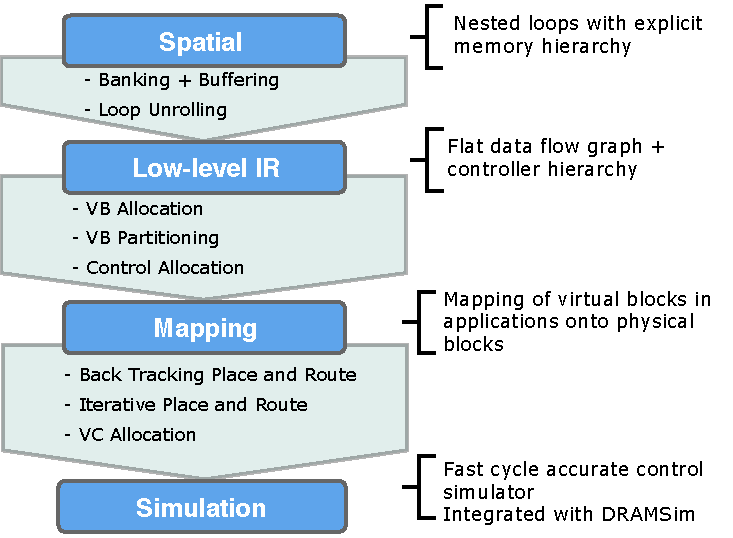
\includegraphics[width=1\linewidth]{figs/flow.pdf}\\
    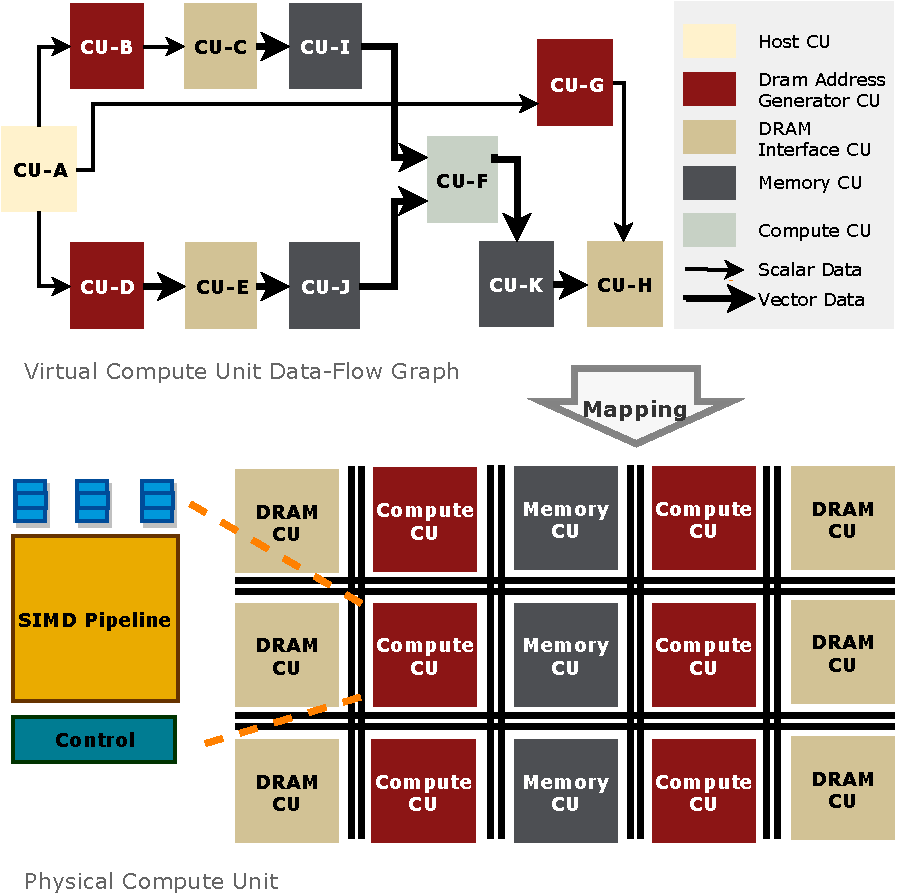
\includegraphics[width=1\linewidth]{figs/mapping.pdf}\\
  }
}
\splitcol{0.6666\columnwidth}{
  \rulebox{Hybrid Networks}{
  }
  \splitcol{0.49\columnwidth}{
    \textbox{
      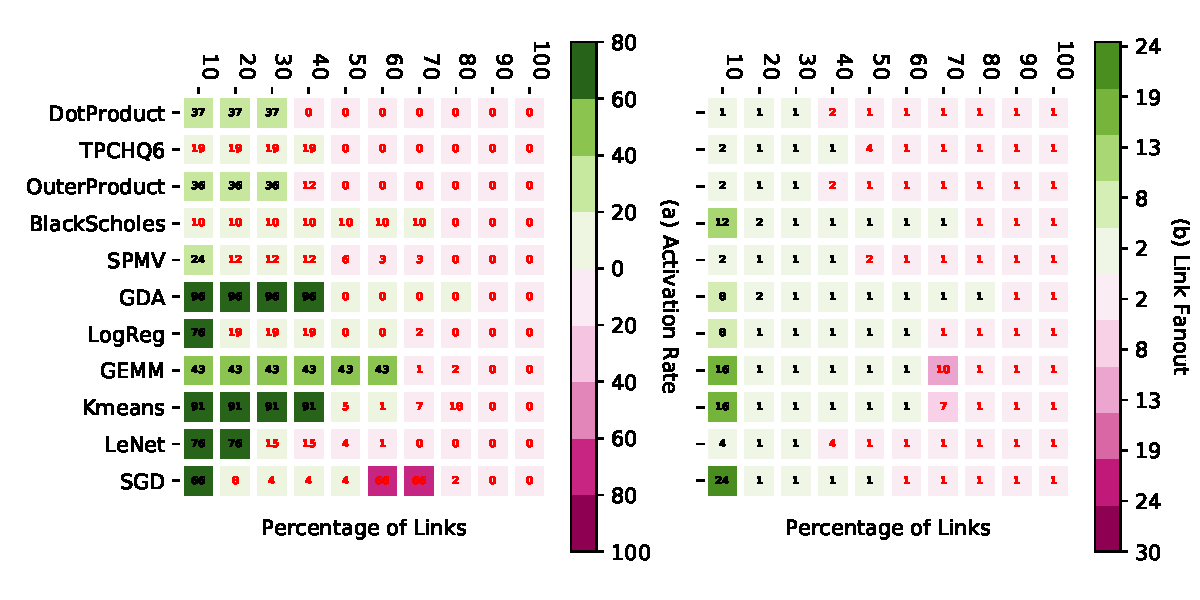
\includegraphics[width=1\linewidth]{figs/link5.pdf}\\
    }
  }
  \splitcol{0.49\columnwidth}{
    \textbox{
      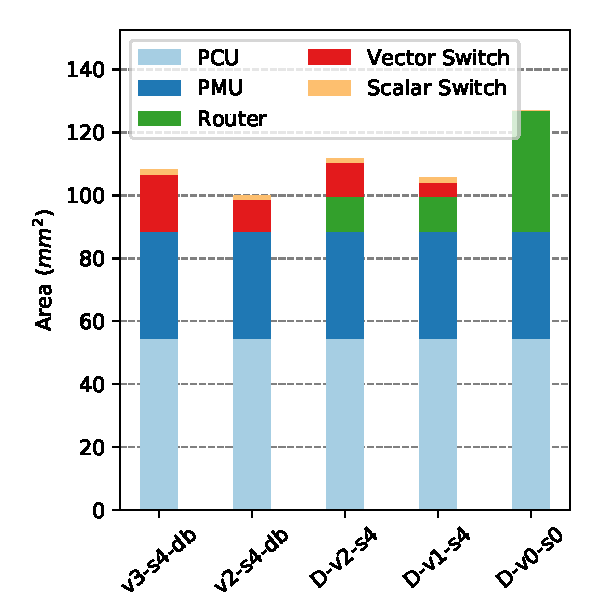
\includegraphics[width=1\linewidth]{figs/area.pdf}\\
    }
  }
  \centering
  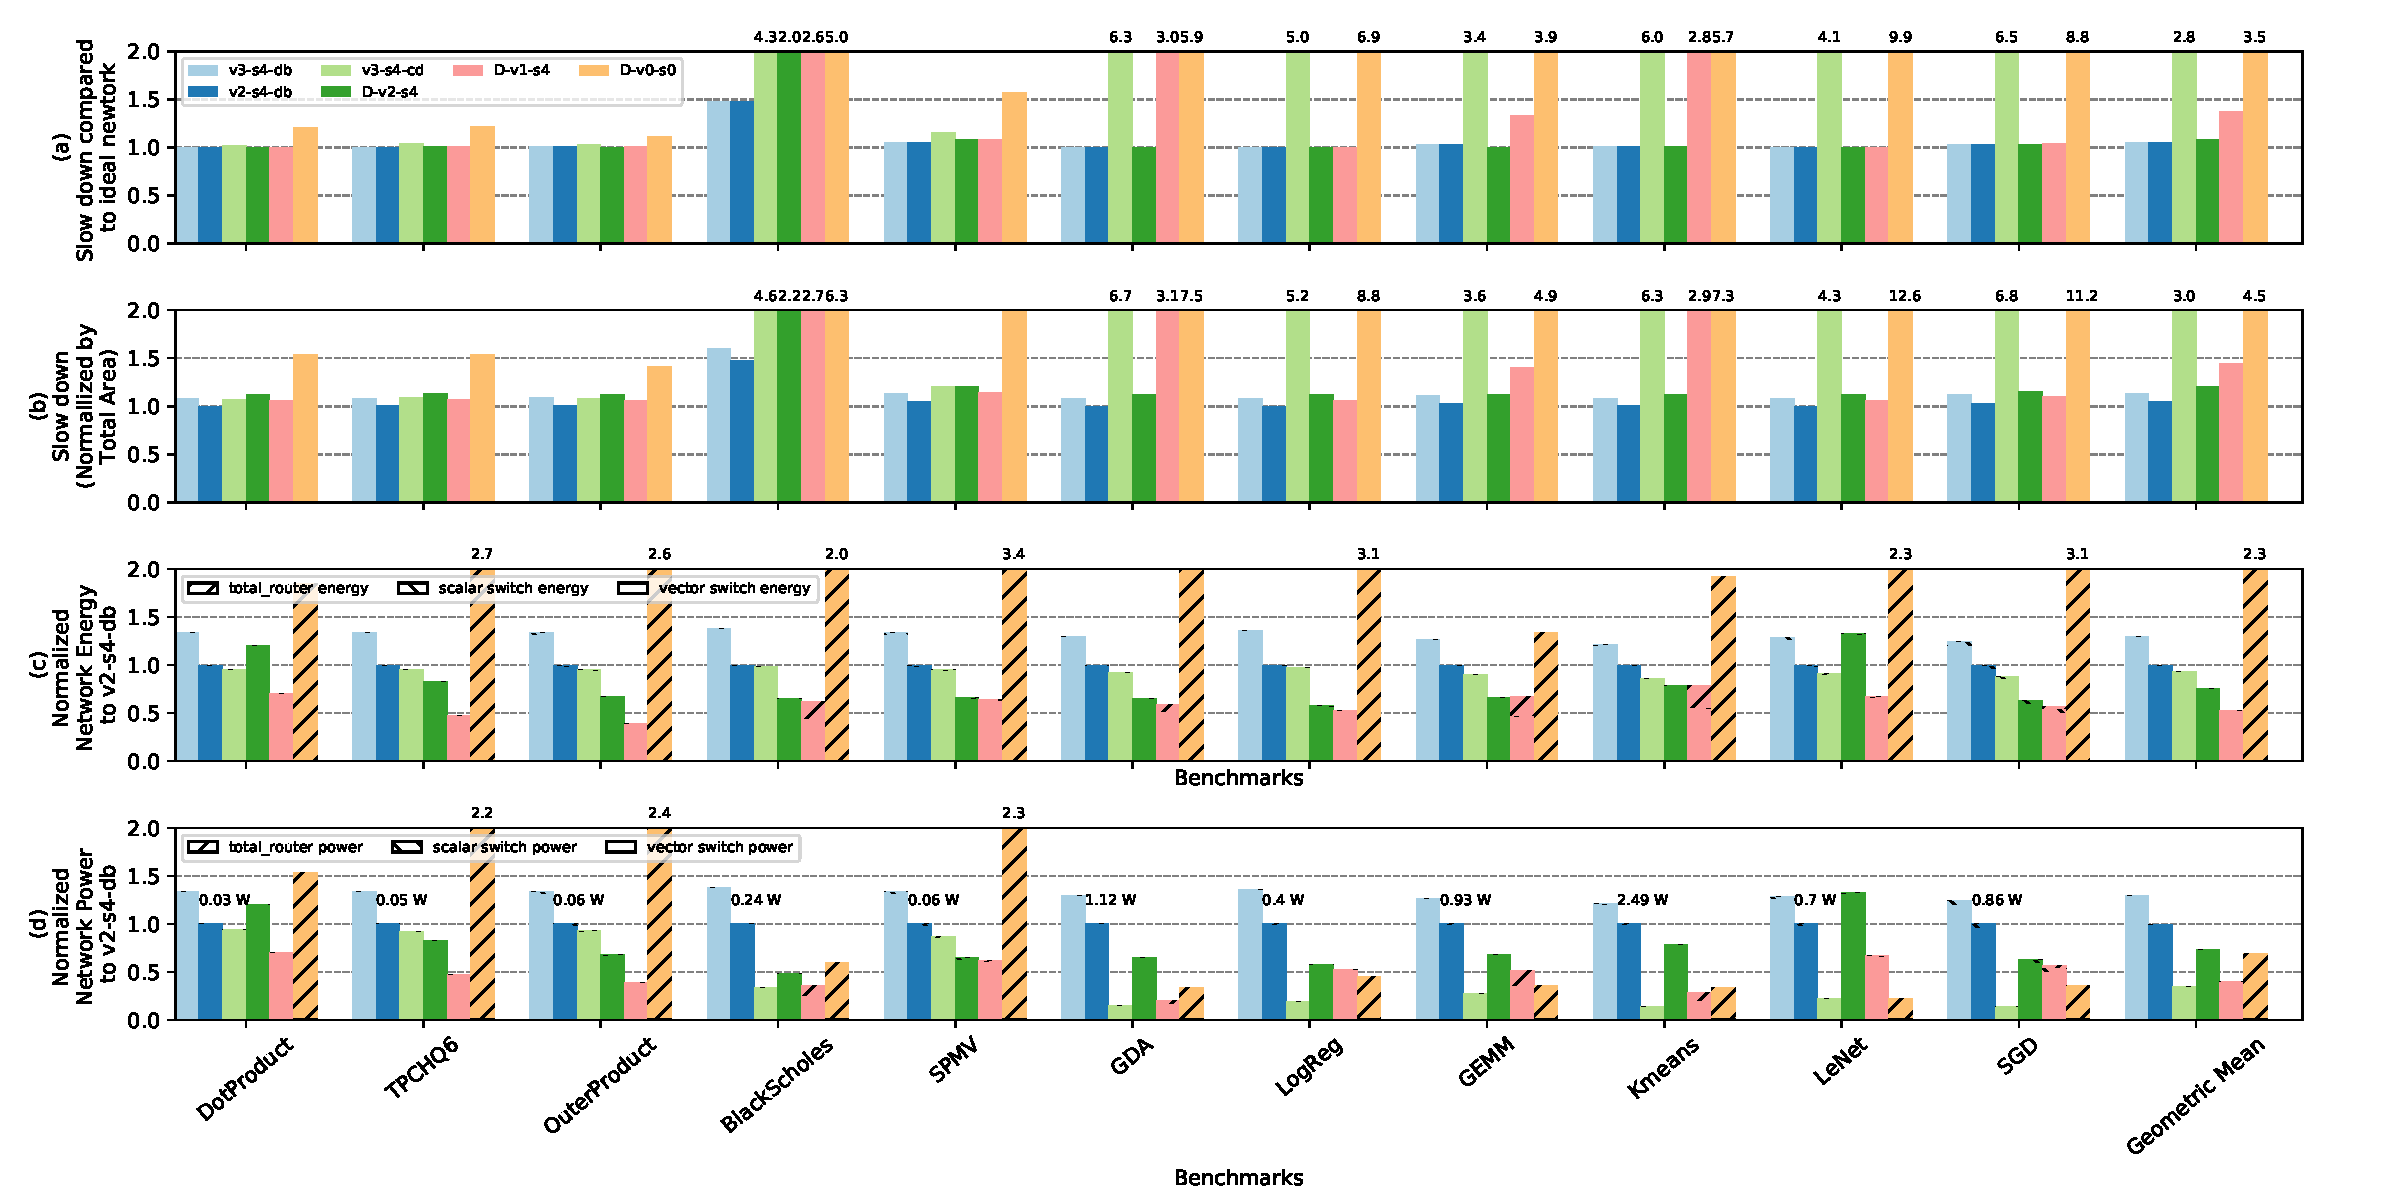
\includegraphics[width=0.7\linewidth]{figs/slow_down.pdf}\\
  \splitcol{0.5\columnwidth}{
  }
  \splitcol{0.5\columnwidth}{
    \centering
    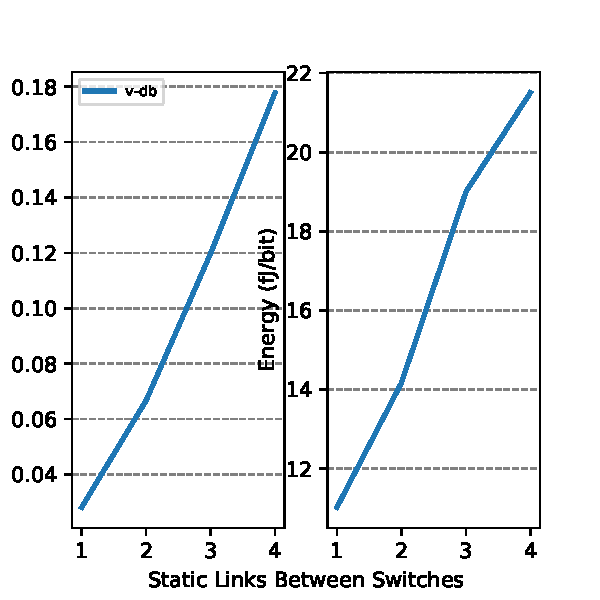
\includegraphics[width=1\linewidth]{figs/switch.pdf}\\
    %\begin{tabular}{cccc}
      %\#VC & Buffer Slots & Area ($\mu m^2$) & Energy($fJ$/bit) \\\hline
      %4 & 2 & 72426.39 & 31.19 \\
2 & 4 & 70390.01 & 28.44 \\
4 & 4 & 127695.32 & 36.11 \\
8 & 4 & 241833.85 & 52.47 \\

    %\end{tabular}\\
  }
  %\splitcol{0.5\columnwidth}{
    %\textbox{
      %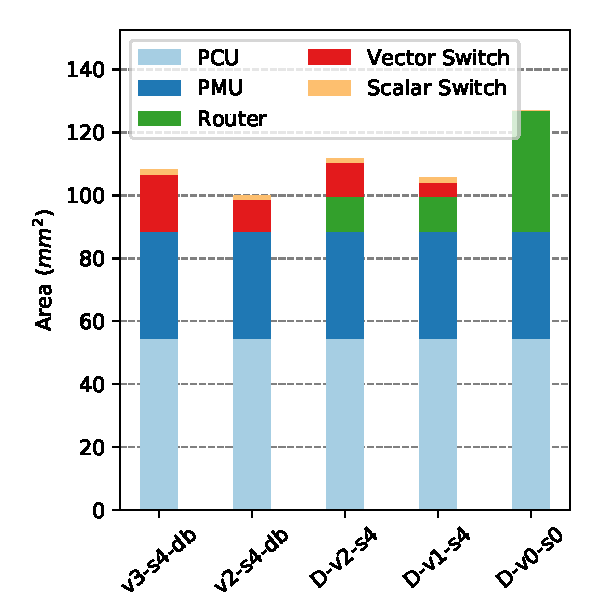
\includegraphics[width=1\linewidth]{figs/area.pdf}\\
    %}
  %}
}

\end{document}
